\section{Problem and Motivation}
\label{sec:problem}
\subsection{Label-Constrained Nearest Neighbors}
Let $\dataset=\{(x_i,A_i)\}_{i=1}^{N}$, with $x_i\in\mathbb{R}^d$ and
finite, nonempty observed label sets $A_i$ (the scope accepted by the
current Trie implementation).  Query $(q,Q,K)$ asks for the $K$ nearest vectors in
\begin{equation}
  \eligible(Q)=\{i:Q\subseteq A_i\},\qquad s(Q)=|\eligible(Q)|/N.
\end{equation}
The distance function is fixed across compared methods.  For workloads with
at least $K$ eligible points, Recall@$K$ is the intersection of the returned
and exact filtered top-$K$ sets, divided by $K$.  If fewer than $K$ points are
eligible, an implementation must instead return at most that number and use
that eligible count as the denominator; an empty eligible set has no ANN
ranking task.  The measured workloads use $K=10$ and exact containment ground
truth.  Query $Q=\varnothing$ is valid and admits all vectors.

Every distinct observed label set $S$ defines an exact group
$G_S=\{i:A_i=S\}$.  Let $G$ denote the number of such groups, distinct from
the vector count $N$.  Labels are unique within a set and sorted under one
fixed total order.  The canonical label trie stores this sequence; its
terminals represent observed groups.  A group-level edge describes permitted
navigation between groups.  Materializing it as vector edges is a separate
construction step, so group-edge counts are not vector-edge counts.

\subsection{An Application Example}
Consider a catalog in which $a$ denotes English, $b$ denotes books, and $c$
denotes in-stock.  A semantic query constrained to books has $Q=\{b\}$.
Groups $\{b\}$, $\{a,b\}$, and $\{a,b,c\}$ are eligible; group $\{a,c\}$ is
not.  Under order $a<b<c$, the first two eligible groups lie on different
prefix branches.  UNG's minimal-superset entry set contains only $\{b\}$,
because set-containment edges can reach the larger groups.  A prefix graph
needs both $\{b\}$ and $\{a,b\}$ as entries.  Removing the second entry would
remove an entire eligible branch from graph-level coverage.

Conversely, a block rooted at prefix $\{a,b\}$ may safely join the
$\{a,b\}$ and $\{a,b,c\}$ groups for query $\{b\}$.  Query $\{b,c\}$ cannot
certify that same block; it must use a finer representation containing the
eligible $\{a,b,c\}$ group.  This is the reason for two granularities: block
size trades geometric freedom against the strength of the predicate
certificate, rather than permitting filter violations inside large blocks.

\begin{figure}[t]
\centering
\begin{tikzpicture}[font=\footnotesize,>=Latex,
 g/.style={draw,rounded corners,inner sep=4pt},
 yes/.style={g,fill=blue!9}, no/.style={g,fill=gray!12}]
\node[yes] (b) at (0,1.6) {$\{b\}$};
\node[yes] (ab) at (2.0,1.6) {$\{a,b\}$};
\node[yes] (abc) at (2.0,0.25) {$\{a,b,c\}$};
\node[no] (ac) at (4.0,1.6) {$\{a,c\}$};
\draw[->,thick] (ab) -- node[right]{prefix} (abc);
\draw[->,dashed,orange!80!black] (b) -- node[above]{LNG only} (ab);
\draw[->,dashed,orange!80!black] (ac) -- (abc);
\draw[blue!60,dotted,thick] (1.12,-0.27) rectangle (2.9,2.05);
\node[align=center] at (2,-0.68) {certifiable block $R_b=\{a,b\}$};
\node[align=center] at (0,-0.05) {separate\\prefix entry};
\end{tikzpicture}
\caption{Illustrative label relations for $Q=\{b\}$. Blue groups are
eligible; the gray group is not. The prefix frontier contains both top blue
groups. Dashed LNG relations and the dotted block boundary explain different
mechanisms; the drawing is not a measured vector layout.}
\label{fig:running-example}
\end{figure}

\subsection{Where Existing Organizations Spend Work}
A global proximity graph, a label-partitioned index, a containment graph, and
a filter-first scan pay for different work.  Figure~\ref{fig:motivation}
summarizes these organizations.  It is not a ranking of implementations.
With a global graph, sparse eligible vertices can force extra traversal or
neighborhood expansion; richer construction may alleviate the problem.
With label-specialized partitions, queries must identify and combine suitable
partitions.  Curator's clustering-based virtual indexes address this
explicitly~\cite{jin2026curator}; a temporary index is not evidence of a
large distance-computation cost by itself.  With UNG, entry discovery and
fine-group traversal both remain relevant.  Filter-first exact scanning has
$\Theta(|\eligible(Q)|d)$ distance work even when the fraction $s(Q)$ is
small, because a large database can still yield many eligible vectors.

\begin{figure*}[t]
\centering
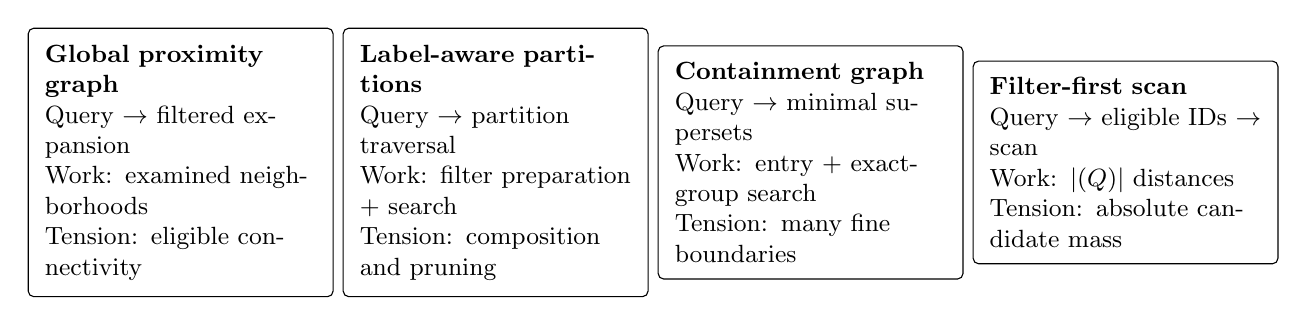
\begin{tikzpicture}[font=\small,
 p/.style={draw,rounded corners=2pt,align=left,text width=3.45cm,
 minimum height=2.0cm,inner sep=6pt}]
\node[p] at (0,0) {\textbf{Global proximity graph}\\
Query $\to$ filtered expansion\\
Work: examined neighborhoods\\
Tension: eligible connectivity};
\node[p] at (4.0,0) {\textbf{Label-aware partitions}\\
Query $\to$ partition traversal\\
Work: filter preparation + search\\
Tension: composition and pruning};
\node[p] at (8.0,0) {\textbf{Containment graph}\\
Query $\to$ minimal supersets\\
Work: entry + exact-group search\\
Tension: many fine boundaries};
\node[p] at (12.0,0) {\textbf{Filter-first scan}\\
Query $\to$ eligible IDs $\to$ scan\\
Work: $|\eligible(Q)|$ distances\\
Tension: absolute candidate mass};
\end{tikzpicture}
\par\smallskip
\begin{tabular}{llrrr}
\toprule
Mean selectivity & 0L system & Discovery (ms) & Seed setup (ms) & Graph (ms)\\
\midrule
0.499\% & LNG + optimized LNG entry & 20.352 & 0.195 & 2.076\\
            & Trie + prefix-frontier entry & 0.645 & 1.769 & 0.868\\
9.907\% & LNG + optimized LNG entry & 36.631 & 0.646 & 98.747\\
            & Trie + prefix-frontier entry & 3.778 & 14.744 & 323.081\\
\bottomrule
\end{tabular}
\caption{Top: conceptual sources of work, not measured shortcomings of
every system in each class. Bottom: measured per-query stage times from the
separate Amazon profile at each system's Recall crossing. Both bases use
their matched entry provider, so this is a system comparison. Timings include
instrumentation and concurrency effects; they are not the batch latency used
to compute primary QPS. The measured rows quantify only the two matched 0L systems.}
\label{fig:motivation}
\end{figure*}

UNG's LNG is the cover graph of observed strict set containment:
$S\to S'$ if $S\subset S'$ and no observed label set is strictly between
them.  It uses a trie to discover minimal observed supersets; that lookup
trie does not define its cross-group edges.  Our prefix instance changes both
the group relation and the matching entry contract.  Our block overlays then
change the navigation unit.  These interventions must be measured separately:
neither a faster entry routine nor fewer group edges alone establishes a
faster filtered nearest-neighbor index.
